{\color{gray}\hrule}
\begin{center}
\section{Model Results}
\textbf{Validating the Model Against Clinical Trials}
\bigskip
\end{center}
{\color{gray}\hrule}

\subsection{Recreating the STEP Trial}
To validate our model's ability to capture the physiological changes induced by semaglutide, we first attempted to recreate the results from the STEP trial. This trial provided detailed biomarker measurements at baseline, 2 weeks, and 2 years, allowing for comprehensive validation of our model's predictions.

The simulation began with a subject matching the trial's baseline characteristics (BMI = 38.79 kg/m$^2$, weight = 105.6 kg) and tracked nine key biomarkers over the 2-year treatment period. Through binary search optimization, we determined that the pre-treatment caloric intake was 3,258 kcal/day, which decreased to 2,678 kcal/day during treatment.

\begin{figure}[h]
\centering
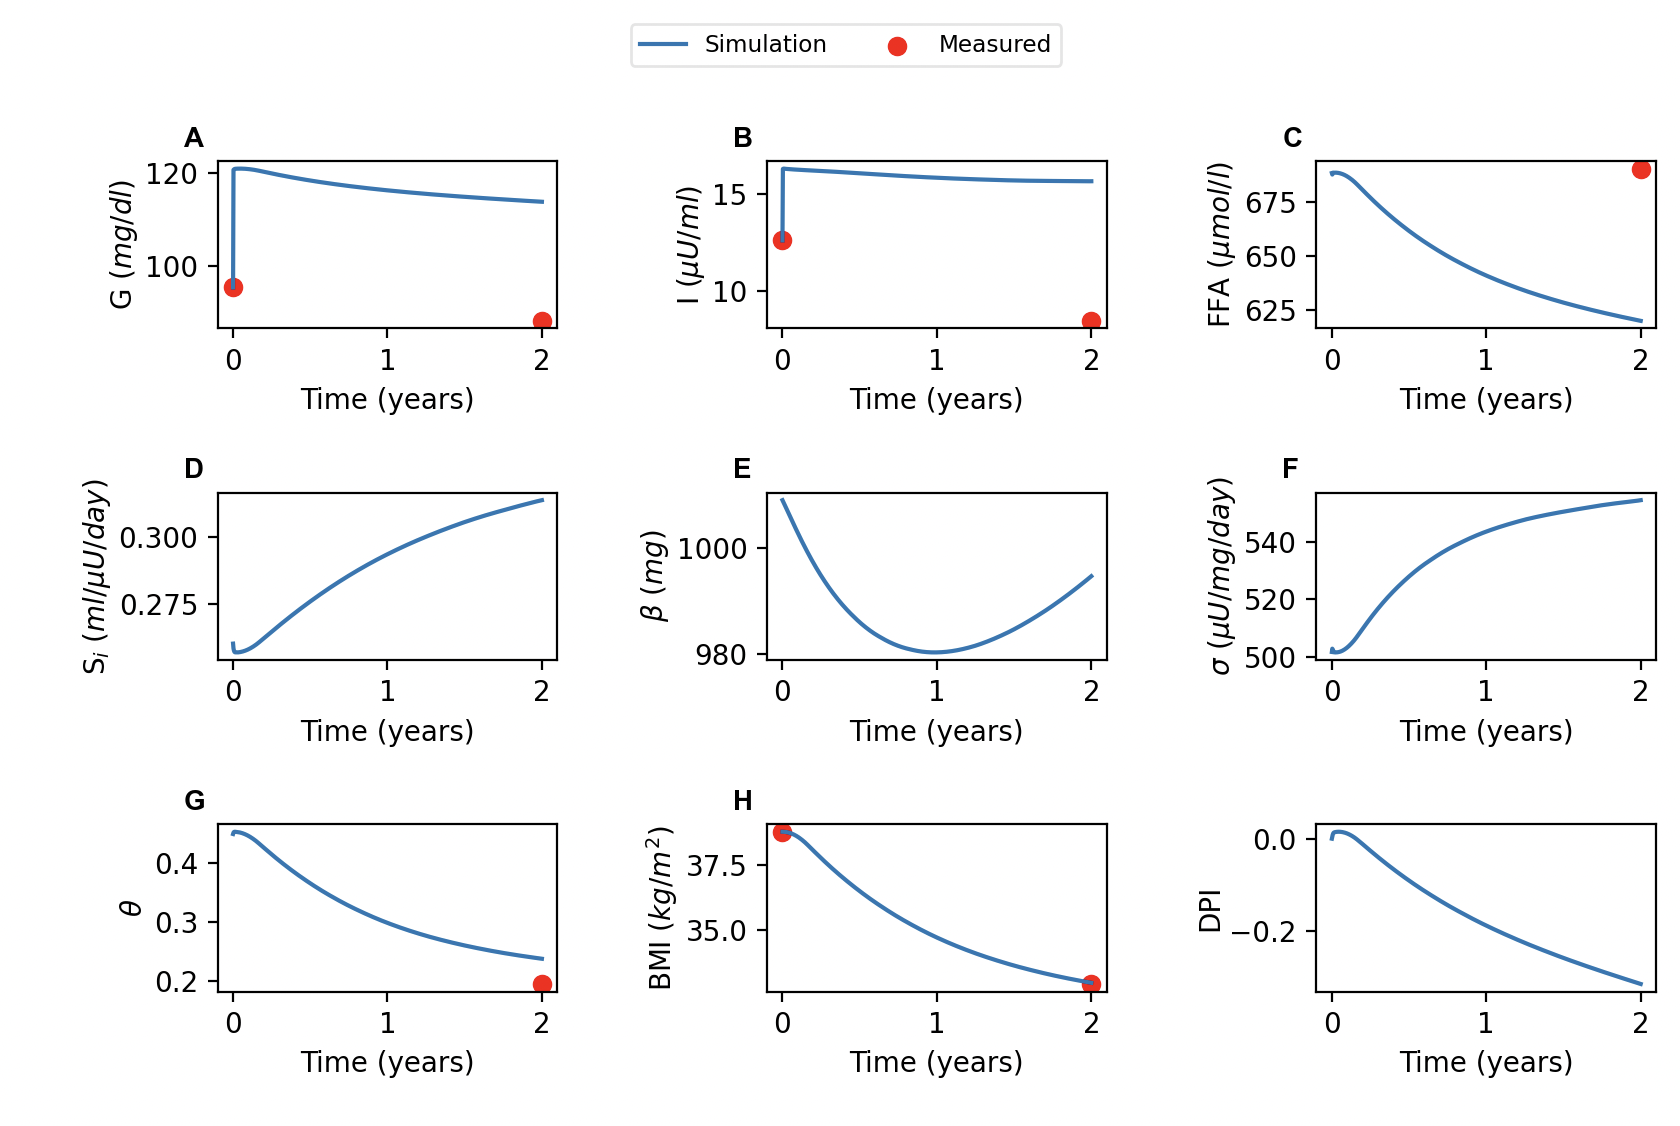
\includegraphics[width=0.95\textwidth]{images/step_trial_simulations.png}
\caption{Temporal evolution of nine key biomarkers during semaglutide treatment in the STEP trial. Blue lines represent model simulations while red dots show measured clinical data.}
\label{fig:step_trial}
\end{figure}

Figure \ref{fig:step_trial} shows the temporal evolution of these biomarkers, revealing several notable patterns and discrepancies:

\begin{itemize}
    \item \textbf{Glucose Dynamics (Panel A):} The model predicted significantly higher glucose levels than measured, showing an immediate jump from 95.4 mg/dl to 121.0 mg/dl, despite the measured baseline being lower. This suggests our model may overestimate initial glucose responses to treatment.
    
    \item \textbf{Insulin Response (Panel B):} Similar to glucose, the model predicted higher insulin levels than observed, jumping from 12.6 $\mu$U/ml to 16.3 $\mu$U/ml at treatment initiation. This consistent overestimation suggests potential refinements needed in our insulin response parameters.
    
    \item \textbf{Free Fatty Acids (Panel C):} While our model predicted a substantial decrease in FFA levels (from 688.7 to 619.7 $\mu$mol/l), clinical measurements showed a slight 0.3\% increase. This discrepancy warrants further investigation into our FFA metabolism assumptions.
    
    \item \textbf{Insulin Sensitivity (Panel D):} S$_i$ showed gradual improvement from 0.26 to 0.31 ml/$\mu$U/day, though without clinical measurements for validation.
    
    \item \textbf{Beta Cell Mass (Panel E):} The model predicted an initial decline followed by partial recovery, stabilizing around 994.6 mg. While plausible, direct validation was not possible as beta cell mass cannot be measured in vivo.
    
    \item \textbf{Insulin Secretion (Panel F):} Predicted increase from 501.6 to 554.7 $\mu$U/mg/day aligns with expected compensatory responses to treatment.
    
    \item \textbf{Inflammation (Panel G):} The model's predicted 46.7\% reduction in inflammation (0.45 to 0.24) closely matched the observed 56.7\% decrease, providing strong validation of our inflammation dynamics.
    
    \item \textbf{BMI (Panel H):} The model accurately captured the reduction from 38.79 to 32.94 kg/m$^2$, matching clinical measurements at both baseline and endpoint.
    
    \item \textbf{Disposition Index (Panel I):} The steady improvement in DPI (reaching -0.32) suggests enhanced glucose homeostasis, though direct clinical validation was not available.
\end{itemize}

These results demonstrate both strengths and limitations of our model. While it accurately captures long-term weight loss and inflammation reduction, the acute metabolic responses (particularly glucose and insulin) may require refinement. The model's predictions for unmeasurable parameters (beta cell mass, insulin sensitivity) appear physiologically plausible but would benefit from indirect validation through additional biomarkers.

\subsection{Recreating the STASIS Trial}
Our stasis model simulated treatment outcomes across four BMI categories ($<$30, 30-35, 35-40, and $\geq$40), with a 5-year disease progression period followed by treatment. While the STASIS trial only provided weight change validation data, our simulation offers hypothetical insights into broader metabolic dynamics, albeit with important limitations noted from our STEP trial validation.

\begin{figure}[!h]
\centering
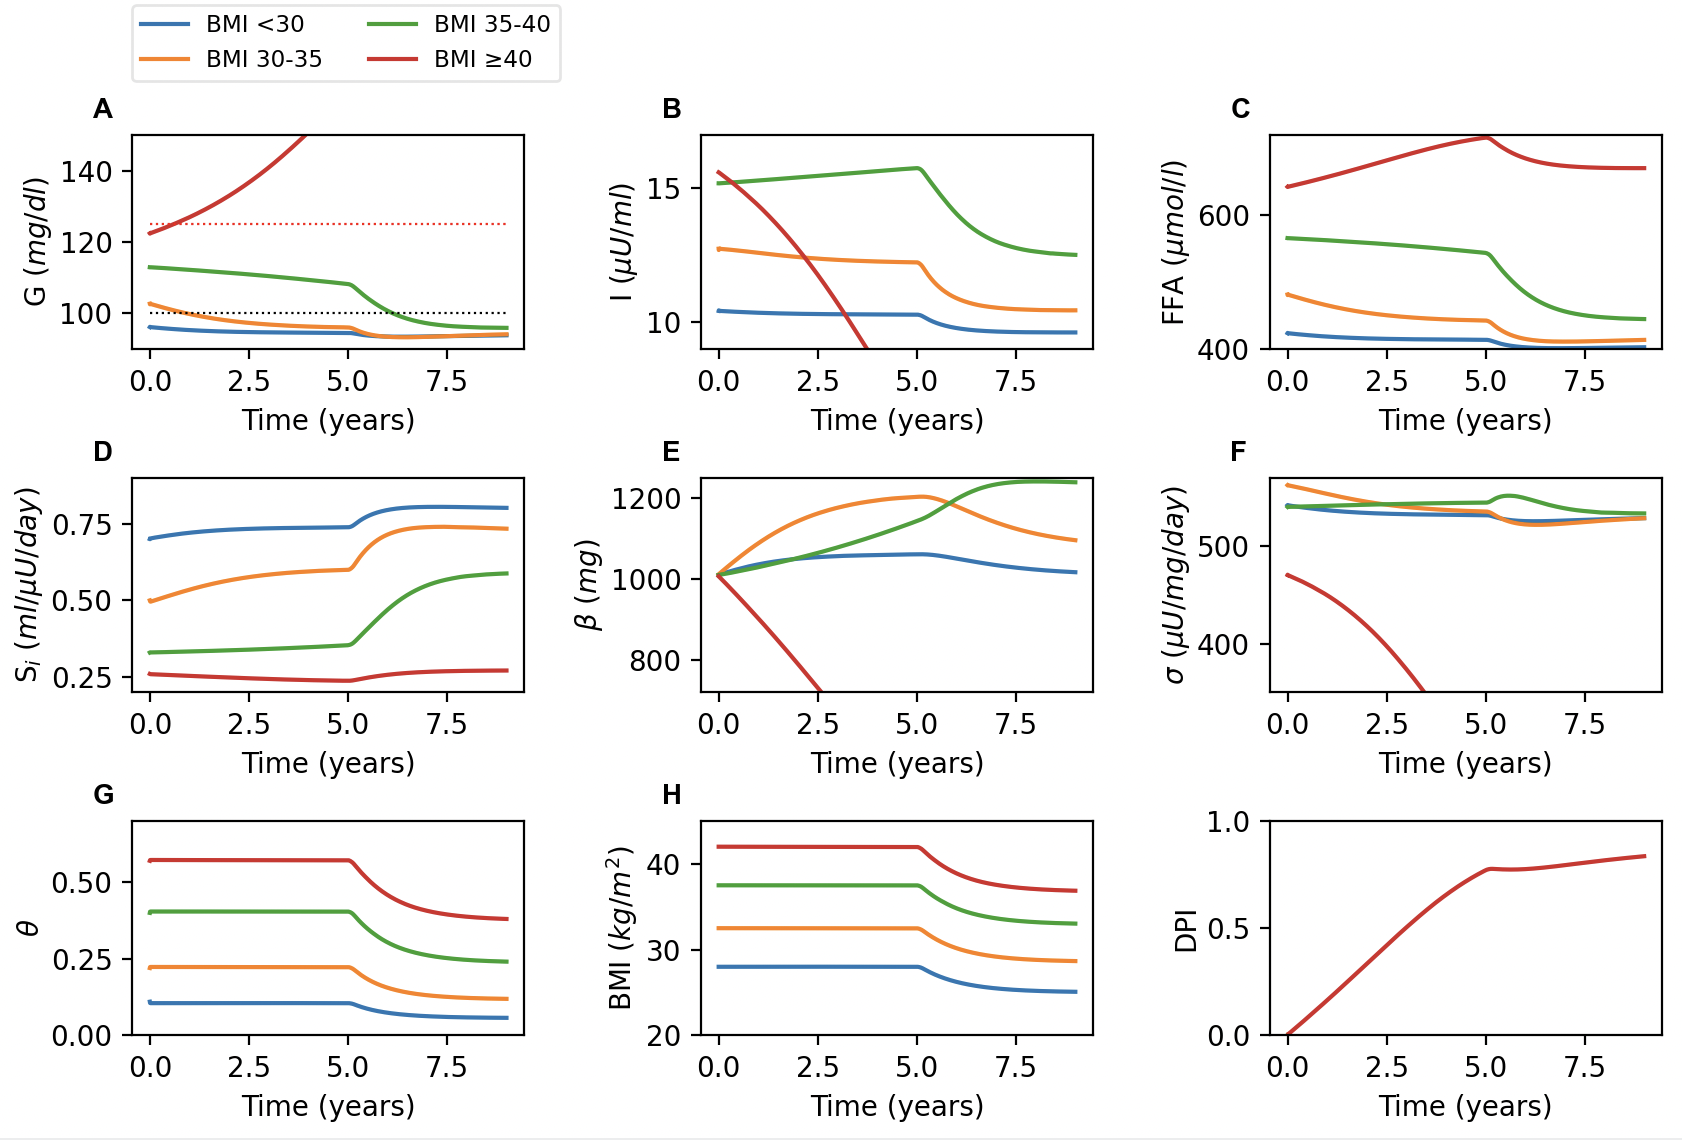
\includegraphics[width=0.95\textwidth]{images/stasis_trial_simulations.png}
\caption{Temporal evolution of biomarkers across BMI groups during simulated disease progression (0-5 years) and treatment (5-7.5 years).}
\label{fig:stasis_trial}
\end{figure}

Analysis by panel reveals distinct patterns across BMI groups:

\begin{itemize}
    \item \textbf{Glucose Dynamics (Panel A):} While lower BMI groups ($<$40) maintained relatively stable glucose levels, the BMI $\geq$40 group showed concerning progression to severe hyperglycemia ($>$160 mg/dl) that persisted through treatment. However, this prediction likely overestimates glucose dysfunction, as clinical evidence shows GLP-1 medications can effectively normalize glucose in higher BMI patients through mechanisms beyond caloric restriction.
    
    \item \textbf{Insulin and FFA Levels (Panels B, C):} The model shows divergent patterns between BMI groups, with particularly concerning drops in insulin for BMI $\geq$40. Given our STEP validation results, these specific predictions should be interpreted with caution.
    
    \item \textbf{Insulin Sensitivity (Panel D):} All groups show gradual improvement during treatment, though the magnitude varies significantly by initial BMI. The BMI $\geq$40 group shows minimal recovery, suggesting a potential ``point of no return'' in our model that may not reflect clinical reality.
    
    \item \textbf{Beta Cell Mass (Panel E):} A striking feature is the dramatic beta cell mass deterioration in the BMI $\geq$40 group, contrasting with stable or increasing mass in lower BMI groups. This prediction appears overly pessimistic given clinical observations of metabolic recovery in high-BMI patients.However, it is plausible under the assumption that the patient is only doing calorie restriction and not semaglutide.
    
    \item \textbf{Insulin Secretion (Panel F):} The model suggests severely compromised insulin secretion in the highest BMI group, while other groups maintain relatively stable function. This stark difference likely overestimates the irreversibility of beta cell dysfunction.
    
    \item \textbf{Inflammation (Panel G):} All groups show improvement with treatment, though the magnitude of reduction correlates with initial BMI. This general pattern aligns with expected inflammatory responses to weight loss.
    
    \item \textbf{BMI Trajectories (Panel H):} The model captures differential weight loss patterns across groups, with higher initial BMIs showing larger absolute reductions. This aspect aligns with clinical observations.
    
    \item \textbf{Disease Progression Index (Panel I):} While lower BMI groups show improvement (moving into negative DPI values), the BMI $\geq$40 group maintains positive values, suggesting persistent metabolic dysfunction. This binary distinction likely oversimplifies the continuous nature of metabolic recovery.
\end{itemize}

\textbf{Model Limitations:} A critical limitation of our model is its failure to capture the full therapeutic effects of GLP-1 medications beyond caloric restriction. This is particularly evident in the BMI $\geq$40 group, where our model suggests irreversible metabolic dysfunction that contradicts clinical evidence of successful treatment outcomes. The model appears to overestimate the permanence of beta cell damage and underestimate the capacity for metabolic recovery in severe obesity. Future iterations should incorporate additional GLP-1 mechanisms of action, including direct effects on insulin sensitivity and beta cell function.